\section{K-means codebook}
\label{sec:intro}

We implemented the classification process following the visual codebook pipeline provided in the instruction. First, we extracted 100K SIFT feature descriptors from the training data and applied K-means clustering to construct a visual vocabulary.

%-------------------------------------------------------------------------
\subsection{Vocabulary size of K-means clustering}
Theoretically, a smaller visual vocabulary size $K$ increases the risk of underfitting but offers better time-wise efficiency. Conversely, a larger $K$ poses a higher risk of overfitting and results in lower efficiency. Theoretically, the time complexity of K-means clustering training and vector quantization is proportional to the value of $K$, and our result \cref{fig:q1-fig1} align with it.

\begin{figure}[htbp]
	\centering
	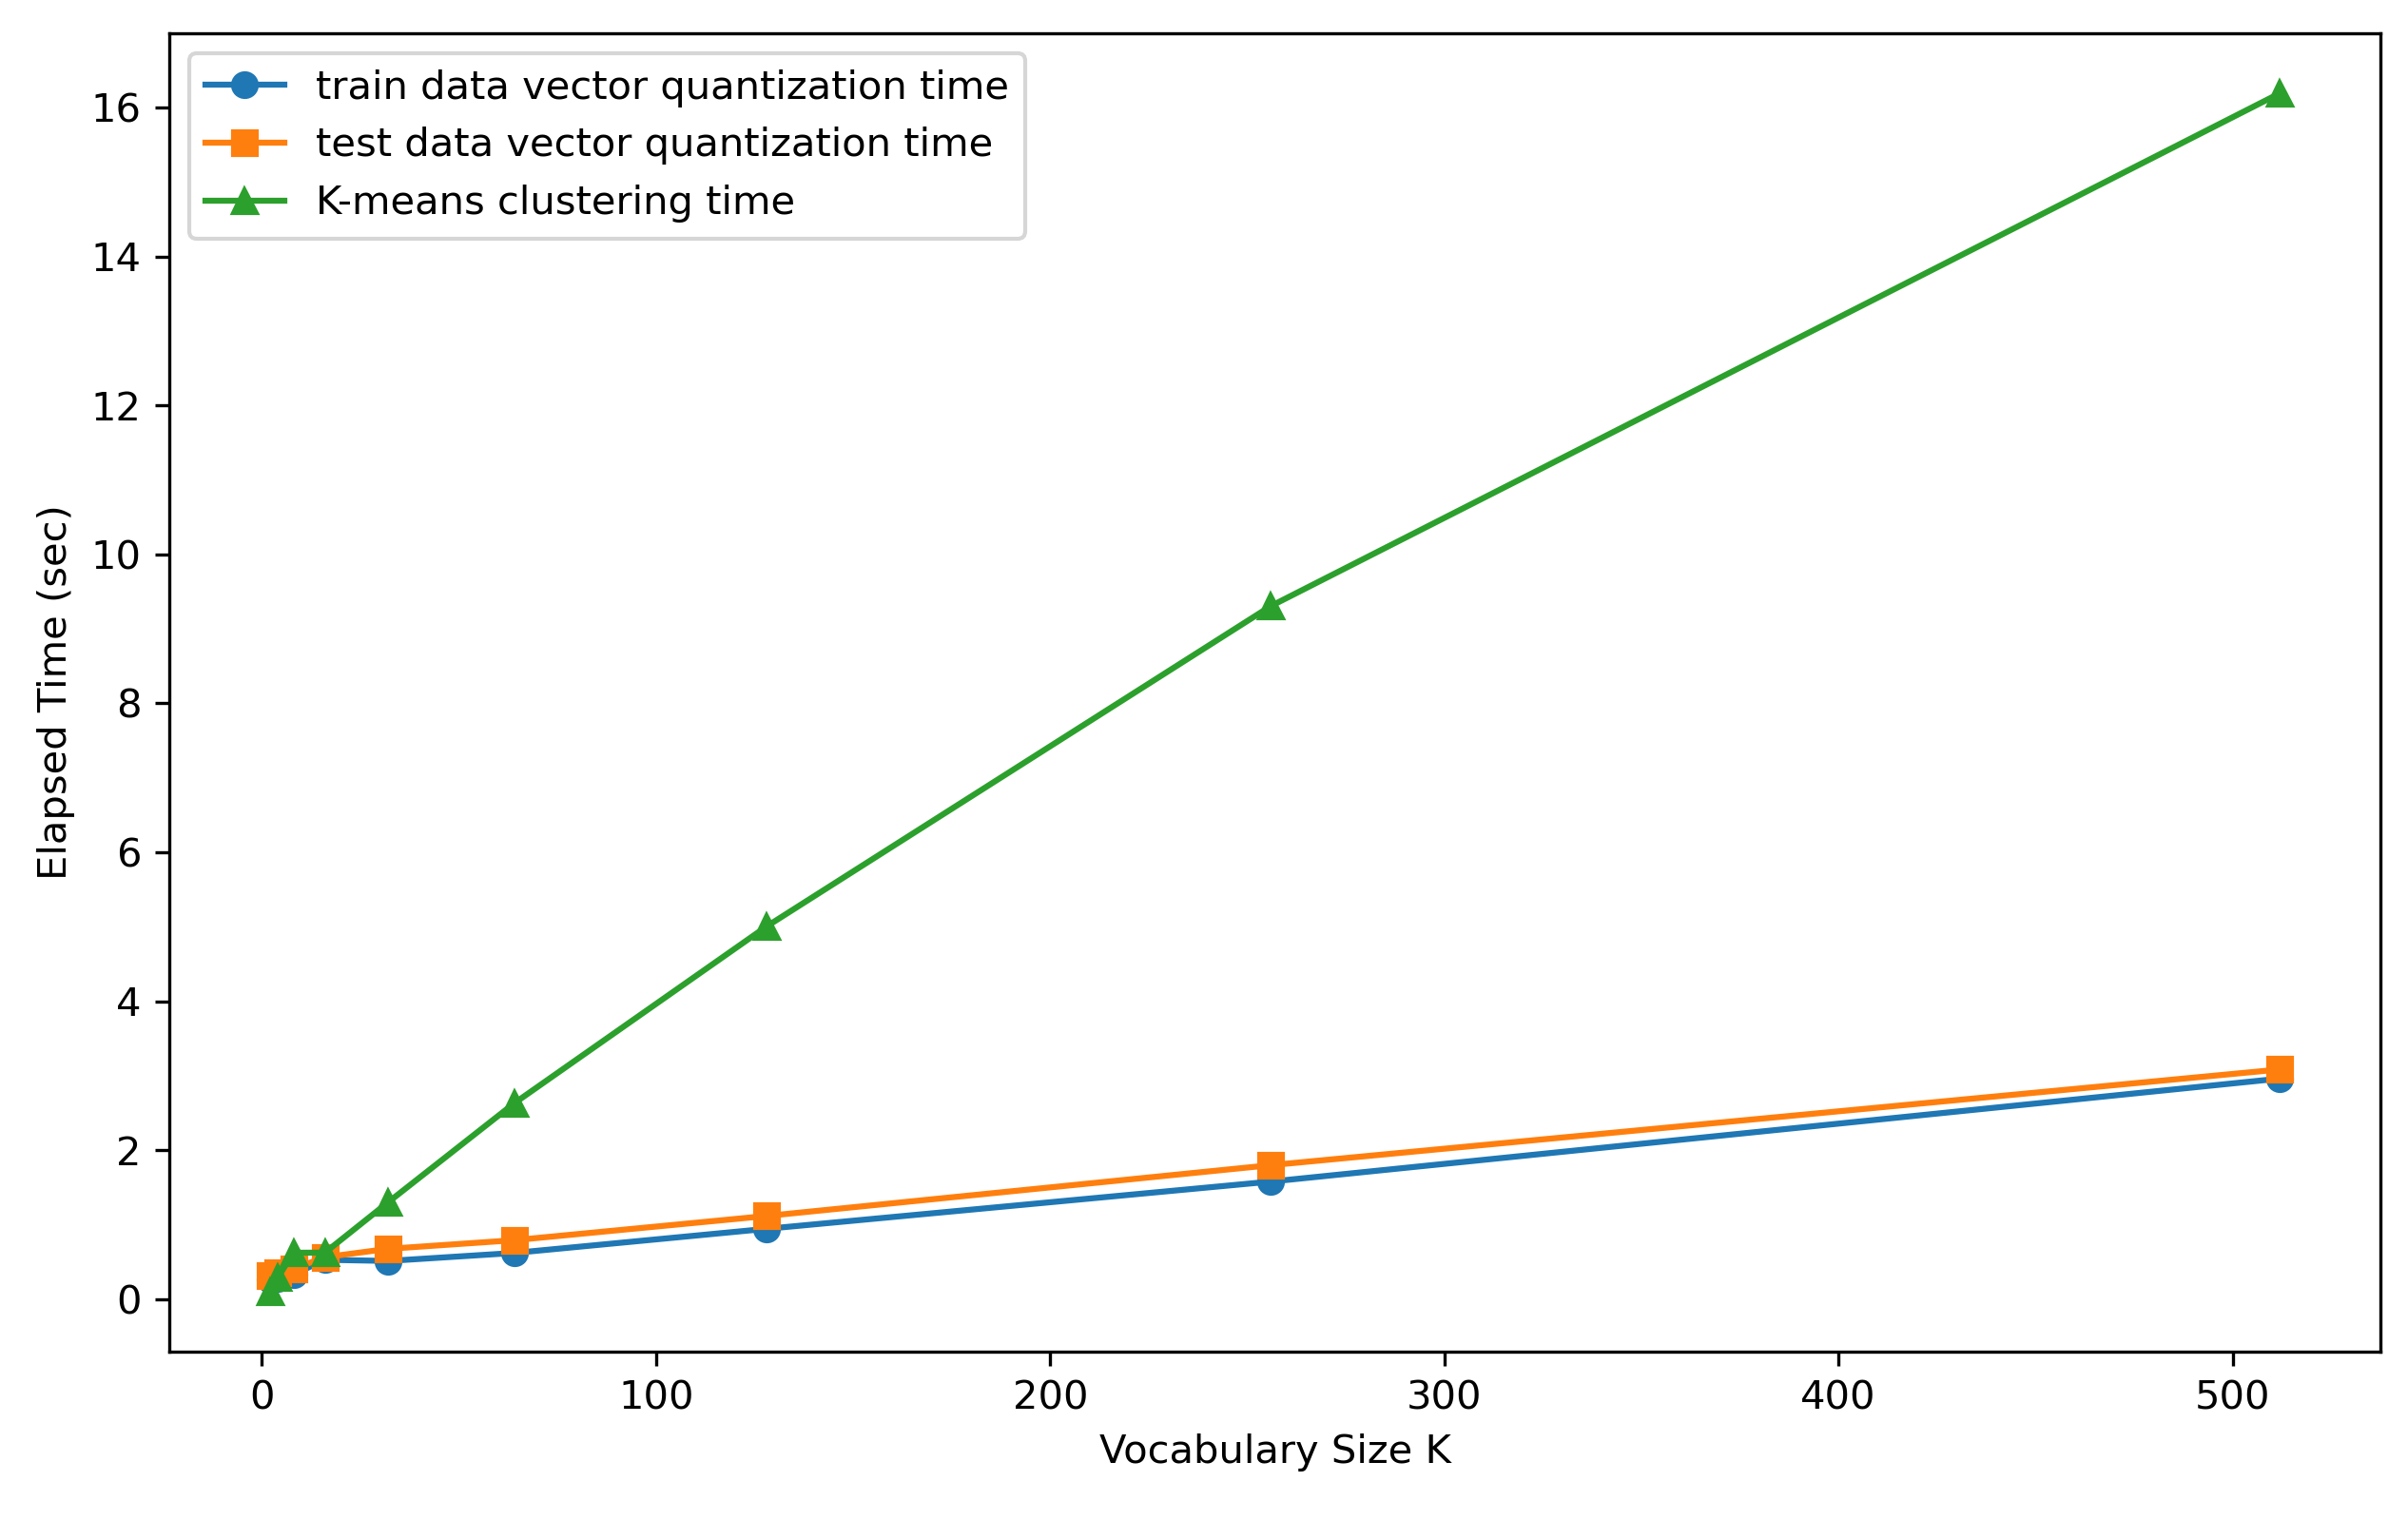
\includegraphics[width=0.5\linewidth]{image/q1-fig1.png}
	\caption{K-means visual vocabulary: training and quantization time according to the value of $k$}
	\label{fig:q1-fig1}
\end{figure}

\subsection{Vector quantisation process}
 To quantize images, the SIFT feature descriptors extracted from each image were assigned to the nearest vocabulary cluster, and a histogram vector was generated based on the vocabulary frequency of such assigning result. Consequently, after vector quantization, the dimension of each image was reduced to the size of visual vocabulary, denoted by $K$. The visualisation result of those histogram 
 